% SCHMT

%%%% TO LATE CROP THE PDF AT THE CORRECT SIZE FOR PLOTING: %%%%
% pdfcrop --margins '-0 -0 -0 -428' scat_HMT.pdf ../scat_HMT_crop.pdf

\documentclass{article}
\usepackage{tikz}
\usetikzlibrary{arrows}

\tikzset{
  treenode/.style = {align=center, inner sep=0pt, text centered,  font=\sffamily},
  % U node: empty black circle text abov
  arn_V/.style = {treenode, circle, blue, draw=black, minimum width=1.5em, font=\tiny}, % font=\sffamily\bfseries
  arn_H/.style = {treenode, circle, white, draw=black, fill=black, minimum width=1.5em, very thick},
  label_U/.style = {node distance=0mm, draw=white, fill=white!20}
  %   arn_x/.style = {treenode, rectangle, draw=black,
%     minimum width=0.5em, minimum height=0.5em}% arbre rouge noir, nil
}

\begin{document}
\hspace*{-35mm}%
	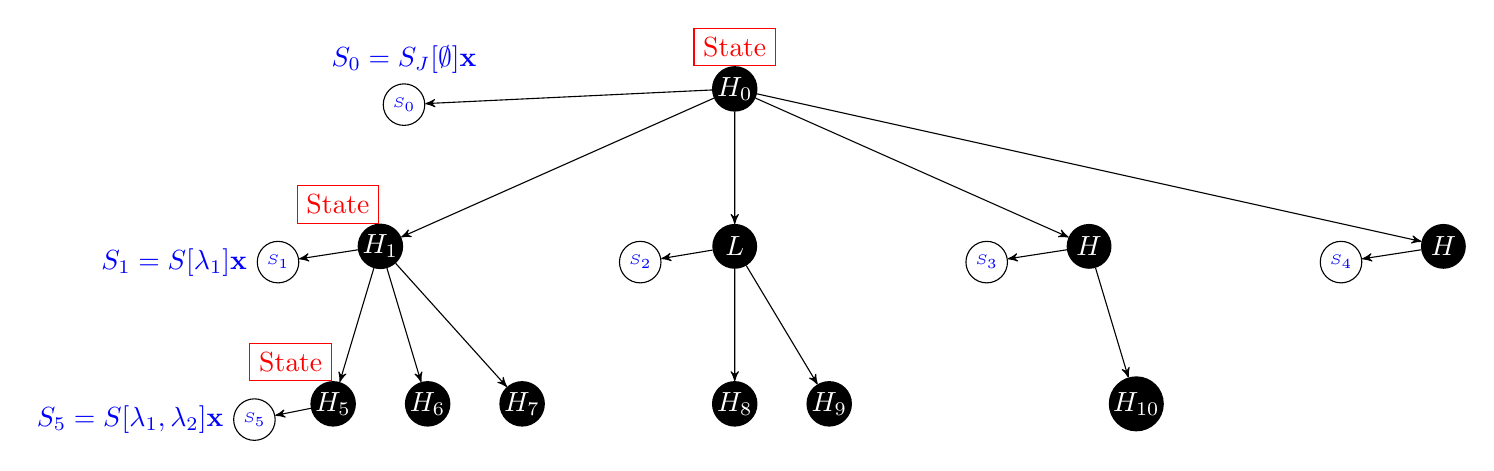
\begin{tikzpicture}[->,>=stealth',
		level 1/.style={sibling distance=45mm, level distance = 2cm},
    level 2/.style={sibling distance=12mm, level distance = 2cm}
    ]
    % Layer 0 - Hidden H_{0}:
		\node [arn_H][label={[draw=red]above:{\color{red}State}}]{$H_{0}$}[xshift=-10mm, yshift=+0mm] 
			% Layer 0 - visible S_{0}:
			child{node [arn_V][xshift=+48mm, yshift=+18mm]
												[label=above:{\color{blue}$S_{0} = S_{J}[\emptyset]\mathbf{x}$}]{$S_{0}$}}
			% Layer 1 - hidden H_{1}:
			child{node [arn_H][label={[draw=red, distance=00mm]93:{\color{red}State}}]{$H_{1}$}  
				% Layer 1 - visible S_{1}:
				child{node [arn_V][xshift=+5mm, yshift=+18mm]
													[label={left:{\color{blue}$S_{1} = S[\lambda_{1}]\mathbf{x}$}}]{$S_{1}$}}
				% Layer 2 - hidden H_{5}:
				child{node [arn_H][label={[draw=red, distance=00mm]93:{\color{red}State}}] {$H_{5}$}
					% Layer 1 - visible S_{5}:
					child{node [arn_V][xshift=-10mm, yshift=+18mm]
														[label={left:{\color{blue}$S_{5} =S[\lambda_{1},\lambda_{2}]\mathbf{x}$}}]{$S_{5}$}}
					}
				% Layer 2  - hidden H_{5}:
				child{node [arn_H] {$H_{6}$}}
				% Layer 2  - hidden H_{6}:
				child{node [arn_H] {$H_{7}$}}
			}
			% Layer 1 - hidden H_{2}:
			child{node [arn_H]{$L$}
						% Layer 1 - visible S_{2}:
						child{node [arn_V][xshift=+0mm, yshift=+18mm]{$S_{2}$}}
						% Layer 2  - hidden H_{8}:
						child{node [arn_H] {$H_{8}$}}
						% Layer 2  - hidden H_{9}:
						child{node [arn_H] {$H_{9}$}}
							}
			child{node [arn_H]{$H$}
						% Layer 1 - visible S_{3}:
						child{node [arn_V][xshift=-7mm, yshift=+18mm]{$S_{3}$}}
						% Layer 2  - hidden H_{10}:
						child{node [arn_H] {$H_{10}$}} 
							}
			child{node [arn_H]{$H$}
						% Layer 1 - visible S_{4}:
						child{node [arn_V][xshift=-13mm, yshift=+18mm]{$S_{4}$}}
						}
		; 
	\end{tikzpicture}
\end{document}

% [label=left:{\color{blue}$S_{J}[\lambda_{1},\lambda_{2}]x$}]